\documentclass[12pt,a4paper,german]{article}
\usepackage{geometry}
\geometry{a4paper, top=25mm, left=25mm, right=25mm, bottom=30mm, headsep=10mm, footskip=12mm}
\usepackage[utf8]{inputenc}
\usepackage{babel}
\usepackage{titlepic}
\usepackage{graphicx}
\usepackage{algorithm}
\usepackage{amsmath}
\usepackage{mathptmx}     % Choose Times New Roman
\usepackage[onehalfspacing]{setspace}
\usepackage[noend]{algpseudocode}
\graphicspath{ {./images/} }
\setcounter{tocdepth}{3}

%\author{Severin Fürbringer \and Adrian Stoop} 

\begin{document}
\begin{titlepage}
  \centering
  
\includegraphics[width=0.075\textwidth]{ktzh}\par
  {\scshape\LARGE Berufsmaturitätsschule Zürich \par}
  \vspace{0.5cm}
  {\scshape\Large Berufsmaturitätsarbeit \par}
  {\scshape Technik,  Architektur,  Life  Sciences \par}
  \vspace{1cm}
  {\huge\bfseries Pathfinding-Algorithmen: Einführung und Vergleich mittels einer Webapplikation \par}
  \vspace{0.5cm}
  Oberthema: \textsc{Mobilität} \\
  \vspace{1cm}
  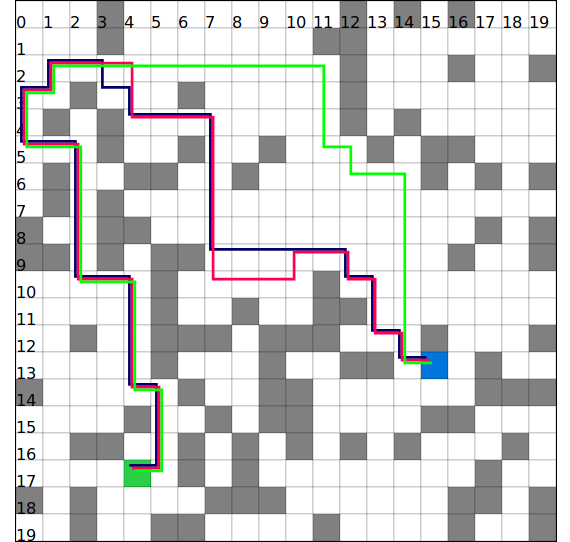
\includegraphics[width=0.5\textwidth]{demo1}\par
  \vspace{1cm}
  \begin{tabular}[t]{c@{\extracolsep{4em}}c} 
    {\Large\itshape Adrian Stoop } & {\Large\itshape Severin Fürbringer } \\
  adrian-stoop@gmx.ch & severin@fsfe.org \\
  EVT18a & EVT18a
  \end{tabular}
  \vfill
  Begleitet von Dr. Jürg \textsc{Pöttinger} \\
  \vfill
  
  % Bottom of the page
  {\large \today \par}
\end{titlepage}
\tableofcontents
\clearpage

\section{Abstract}
Diese Berufsmaturitätsarbeit befasst sich mit der Theorie und Praxis der so genannten Pathfinding Algorithmen (dt. Pfadfindungsalgorithmen) im zweidimensionalen Raum. Deren Grundlegende Idee ist das programmatische Ausrechnen eines Wegplans in einem Strassensystem oder Labyrinth. Die Wirtschaft setzt solche Algorithmen in vielseitigen Anwendung ein. Von Video Spielen bis hin zu höchst komplexen echtzeit Selbstfahrsystemen in der Automobilindustrie.

Es stehen für den Einsatz verschiedene Pathfinding Algorithmen zur Auswahl. Wie diese Algorithmen nahezu magisch ihren eigenen Weg finden, möchten wir anhand einer benutzerfreundlichen Webapplikation näher veranschaulichen. Durch teilweise vorpogrammierte Szenarien lässt sich dann klar verdeutlichen, wie die Pathfinding Algorithmen funktionieren. Schritt zu Schritt spielt die Webapplikation ab, wie ein Pathfinding Algorithmus individuell seinen Weg findet. Paralleler Durchlauf verschiedener Implementationen veranschaulicht ausserdem die visuell erkennbaren Unterschiede und Vor-- und Nachteile. Anhand dieser Folgerungen lässt sich schlussendlich die Theorie mit der Praxis der Webapplikation vergleichen.
\section{Einleitung}
\subsection{Einführung in das Thema}
\subsection{Fragestellung}
\subsection{Hypothese}
\subsection{Inspiration}
\subsection{Visuelle Konzept}
\subsection{Arbeitsmethoden}

\section{Hauptteil}
\subsection{Konzept}
...
\cite[Kapitel X, p.~123]{cuishi2011}

\subsection{Software}
\subsection{Entstehung und Theorie des Pathfinding}

\subsection{Resultate}
\section{Schluss}
\clearpage

\begin{thebibliography}{9}
\bibitem{cuishi2011}
  Xiao Cui and Hao Shi,
  \textit{A*-based Pathfinding in Modern Computer Games},
  IJCSNS International Journal of Computer Science and Network Security, VOL.11 No.1,
  Januar 2011.
\end{thebibliography}
\end{document}
